\usepackage[utf8]{inputenc}
\usepackage[T1]{fontenc}
\usepackage{mathptmx}
\usepackage[scaled=.90]{helvet}
\usepackage{courier}
\usepackage{caption}
\captionsetup{labelformat=empty,labelsep=none}
\usepackage{beamerthemesplit}
\usepackage{verbatim}
\usepackage{hyperref}
\usepackage{listings}
\lstset{language=Perl,basicstyle=\normalsize,tabsize=3,showstringspaces=false}

\title{Wir tanzen um die Welt!}
\author[racke]{Stefan Hornburg (Racke)\\ \texttt{racke@linuxia.de}}
\date{15. Deutscher Perl-Workshop, Berlin, 14. März 2013}

\begin{document}
\maketitle{}

\begin{frame}
  \titlepage
\end{frame}

\tableofcontents

\section{American Spaces}

Die über 850 "American Spaces" weltweit fördern das Verständnis für die Kultur, Politik und den Lifestyle der USA. 

Wir unterstützen die "American Spaces" bei der Beschaffung von Materialien
(Bücher, DVD) und stellen die Infrastruktur für den Zugriff auf öffentlichen
und kommerziellen Datenbanken zur Recherche bereit.

\begin{frame}{American Spaces}
\begin{description}
% Burkina Faso
\item[Ouagadougou] Martin Luther King Jr. Library
% Tonga
\item[Nuku'alofa] American Corner Nuku'alofa

% Simbabwe
\item[Gweru] American Corner Gweru

\end{description}
\end{frame}

\begin{frame}{American Spaces}
\begin{figure}
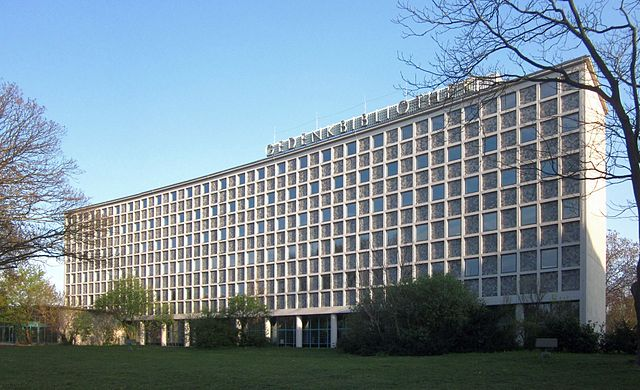
\includegraphics{Amerika-Gedenk-Bibliothek.jpg}
\caption{Amerika-Gedenkbibliothek Berlin}
\end{figure}
\end{frame}

\section{Anwendungen}
    
Die im folgenden vorgestellten Anwendungen sind alle mit Dancer realisiert.
Dancer unterstützt dabei die einfache und schnelle Entwicklung und bietet mit
seinem umfangreichen Ökosystem (Plugins, Hooks, Engines) eine hohe
Flexibilität. Außerdem ist die Dancer-Community sehr aktiv und
hilfsbereit.

Die Daten befinden sich in einem LDAP-Verzeichnis und in
mehreren PostgreSQL-Datenbanken.

\begin{frame}{Anwendungen}
\begin{itemize}
\item Dashboard
\item eShop
\item eLibraryUSA
\item Administration
\item Training
\end{itemize}
\end{frame}

\subsection{Dashboard}
Startpunkt für alle Anwendungen, stellt Single Sign-On zur Verfügung.

\begin{frame}{Dashboard}
\begin{itemize}
\item Homepage intern/extern
\item Single Sign-On (SSO)
\item \url{https://americanspaces.state.gov/}
\end{itemize}
\end{frame}
    
\subsection{eShop}

Der Onlineshop für die "American Spaces" dient zur Beschaffung von
diversen Materialien wie Bücher, DVD, CD, Publikationen.

Daten und Bilder werden teilweise von externen Quellen eingebunden,
wie z.B. ISBNdb.com und LibraryThing.

Die shopspezifischen Daten werden in einer PostgreSQL-Datenbank
verwaltet.

\begin{frame}{eShop}
\begin{itemize}
\item \url{https://eshop.state.gov/}
\item Beschaffung von Materialien
% Bücher, CD, DVD, eBooks, Promomaterial (Poster, Sticker, Postkarten)
\item z.Z. 12 Anbieter
\item Backend für Preise, Ersatztitel
\item Bestpreis
\item Anzeige nur für American Spaces
\end{itemize}
\end{frame}

\begin{frame}{eShop}
\begin{itemize}
\item PostgreSQL
\item ISBNdb.com
\item LibraryThing
\item LiveChat, MailChimp
\item ProForma-Rechnungen mit PDF::WebKit
\end{itemize}
\end{frame}
    
\subsection{eLibraryUSA}

eLibraryUSA gibt Besuchern der American Spaces Zugriff
auf Informationen, die Amerikaner in öffentlichen
Bibliotheken finden können.
    
Die nicht öffentlichen Resourcen werden durch ezProxy zur
Verfügung gestellt. ezProxy greift zur Authentifizierung
der Benutzer auf Single Sign-On mittels HTTPS-Request zu.

\begin{frame}{eLibraryUSA}
\begin{itemize}
\item \url{http://elibraryusa.state.gov/}
\end{itemize}
\end{frame}

\subsection{Training}

Support für Training (Registrierung, Hotel, Material, Kalender)
inklusive Räumlichkeiten in Wien.

\url{https://americanspaces.state.gov/training}
    
\subsection{Administration}

Die Daten zu den American Spaces und den Benutzern werden
mit einer einfachen Administrationsoberfläche bearbeitet.
Die Verantwortlichen vor Ort können für ihren
jeweiligen American Space Benutzer anlegen und pflegen
als auch Informationen über den Space aktualisieren.

\begin{frame}{Administration}
\begin{description}
\item[Spaces] Region, Land, Stadt, GeoIP, ...
\item[Benutzer] Space, Rolle, Email, ...
\end{description}
\end{frame}

\section{LDAP}

Unser LDAP-Verzeichnis beinhaltet die Hierarchie der American Spaces
(Region, Land, Ort) und die Benutzer für unseren Anwendungen.
Außerdem speichern wir Zusatzinformationen zu den American Spaces,
wie z.B. Typ, Homepage, Jahr der Eröffnung, geographische Länge und Breite.
    
Es dient ebenso zur Authentifizierung mittels Single Sign-On, dabei
wird die Emailadresse als eindeutiger Benutzername verwendet.
    
Der Zugriff auf das LDAP-Verzeichnis erfolgt mittels
Dancer::Plugin::LDAP. Dieses Plugin stellt einfache
Methoden bereit, um Einträge zu erstellen, bearbeiten
und umzubenennen.

\begin{frame}[fragile]{Dancer::Plugin::LDAP}
\begin{lstlisting}
ldap->quick_insert("uid=racke@linuxia.de,ou=people," 
                   . ldap->base(),
                   {givenName => 'Stefan',
                    lastName => 'Hornburg',
                    dosInstitute => 'IRC Berlin',
                    dosRole => 'Administrator',
                    c => 'Germany',
                    l => 'Berlin',
                   });
\end{lstlisting}
\end{frame}

Dancer::Plugin::LDAP kümmert sich um die korrekte Behandlung
von UTF-8 und wandelt automatische Attribute ohne Wert in eine
Arrayreferenz mit 0 Elementen um. Da kaum ein LDAP-Attribute einen
leeren String als Wert akzeptiert, würde sonst ein Fehler
ausgelöst.

\section{Single Sign-On (SSO)}

Das Dashboard hat einen SSO-Server integriert und erledigt An- und
Abmeldung sowie das Anlegen und Löschen von Benutzerkontos.

\begin{frame}{Single Sign-On}
\begin{itemize}
\item Anmelden
\item Abmelden
\item Passwort zurücksetzen
\item Passwort ändern
\end{itemize}
\end{frame}

\subsection{Cookies}

Wir verwenden TLD-Cookies. Diese können wie folgt mit Dancer
gesetzt werden:

\begin{frame}[fragile]{Cookies}
\begin{lstlisting}

    cookie 'sso.username' => 'racke@linuxia.de',
           domain => '.state.gov',
           expires => config->{session_expires};

\end{lstlisting}
\end{frame}

Zusätzlich wird ein verschlüsseltes Token vom SSO-Server
erzeugt und mitgeschickt.                       
                       
\subsection{Passwort Policy}

Um die Sicherheit der verwendeten Passwörter zu erhöhen, wird
folgende Policy eingesetzt:

Ein Passwort besteht aus mindestens 8 Zeichen, in denen
ein Klein- und ein Großbuchstabe, eine Ziffer und ein
anderes Zeichen vorkommen muß.

Außerdem wird das Passwort auf typische Muster (1234, qwertz),
Wiederholungen und "Leet" (4tw, m3h, ph34r) geprüft.

\begin{frame}{Passwort Policy}
Data::Transpose::PasswordPolicy
\end{frame}

\subsection{Email-Validierung}

Beim Anlegen der Benutzerkonto wird die Emailadresse
mit Email::Valid überprüft. Dabei wird außer auf
syntaktischen Fehlern in der Emailadresse (racke.linuxia.de)
auch überprüft, ob für die Domain ein DNS-Eintrag (A oder MX)
existiert.    
                   
\begin{frame}{Email-Validierung}
\begin{itemize}
\item Email::Valid
\item mxcheck
\end{itemize}
\begin{itemize}
\item VERP
\end{itemize}
\end{frame}

\section{Entwicklung \& Deployment}

\subsection{Lokale OpenLDAP-Instanz}

Dazu erstellen wir zunächst eine lokale \verb|slapd.conf|. Dann legen
wir das \verb|db|-Verzeichnis an und kopieren \verb|DB_CONFIG| aus dem
Verzeichnis \verb|/usr/share/slapd>| hinein.

Jetzt importieren wir eine LDIF-Datei mit den Livedaten:

    /usr/sbin/slapadd -f slapd.conf live.ldif

Und starten unsere lokale Instanz:

    /usr/sbin/slapd -u 1000 -g 1000 -h ldap://127.0.0.1:9009 -f slapd.conf

\begin{frame}[fragile]{Lokale OpenLDAP-Instanz}
\begin{lstlisting}
% rm -rf ldap/db
% mkdir ldap/db
% cp /usr/share/slapd/DB_CONFIG ldap/db
% /usr/sbin/slapadd -f slapd.conf live.ldif
% /usr/sbin/slapd -u 1000 -g 1000 \
      -h ldap://127.0.0.1:9009 -f slapd.conf
\end{lstlisting}
\end{frame}

\subsection{Email Redirect}

Um nicht versehentlich Emails an echte Benutzer zu versenden,
werden diese zum jeweiligen Entwicker umgeleitet mit
Email::Sender::Transport::Redirect und folgender
Dancer-Konfiguration:

\begin{frame}[fragile]{Email Redirect}
\begin{lstlisting}

    plugins:
      Email:
        transport:
          Sendmail:
            redirect_address: racke@linuxia.de

\end{lstlisting}
\end{frame}

\subsection{Nginx}
    
Wir betreiben Nginx als "Reverse Proxy" und benutzen Starman als
Plack-Backend.

Hier die entsprechende Konfiguration (vereinfacht) für einen virtuellen
Host:

\begin{frame}[fragile]{Nginx-Konfiguration}
\begin{lstlisting}
server {
    listen 80;
    server_name elibraryusa.state.gov;
    root /home/dancer/Elib/public;

    ...
}
\end{lstlisting}
\end{frame}

\begin{frame}[fragile]{Nginx-Konfiguration}
\begin{lstlisting}
server {
    ...

    location / {
        try_files $uri @proxy;
        access_log off;
        expires max;
    }

    ...
}
\end{lstlisting}
\end{frame}

\begin{frame}[fragile]{Nginx-Konfiguration}
\begin{lstlisting}
server {
   ...

   location @proxy {
        proxy_set_header Host $http_host;
        proxy_set_header X-Forwarded-Host $host;
        proxy_set_header X-Real-IP $remote_addr;
        proxy_set_header X-Forwarded-For $proxy_add_x_forwarded_for;
        proxy_pass       http://localhost:5001;
    }
}
\end{lstlisting}
\end{frame}

\begin{frame}[fragile]{Nginx-Konfiguration SSL}
\begin{lstlisting}
server {
   listen 213.129.249.66:443;
   server_name eshop.state.gov;
   root /home/interch/eShop/public;

   ssl on;
   ssl_certificate_key  /etc/ssl/private/eshop.state.gov.key;
   ssl_certificate    /etc/ssl/certs/eshop.state.gov.pem;

   ...
}
\end{lstlisting}
\end{frame}

\begin{frame}[fragile]{Nginx-Konfiguration SSL}
\begin{lstlisting}
server {
   ...

   location @proxy {
        proxy_set_header Host $http_host;
        proxy_set_header X-Forwarded-Host $host;
        proxy_set_header X-Real-IP $remote_addr;
        proxy_set_header X-Forwarded-For $proxy_add_x_forwarded_for;
        proxy_set_header X-Forwarded-Proto https;
        proxy_pass       http://localhost:5001;
    }
}
\end{lstlisting}
\end{frame}

\end{document}

%%% Local Variables: 
%%% mode: latex
%%% TeX-master: t
%%% End: 
